\documentclass[a4paper, twoside, 12pt]{article}
\usepackage[utf8]{inputenc}
\usepackage[T1]{fontenc}
\usepackage{graphicx}
\usepackage{longtable}
\usepackage{hyperref}
\usepackage{caption}
\usepackage{verbatim}
\usepackage{listings}
\usepackage{amsmath,amssymb}

% set margins for double-sided printing
\usepackage[left=2.5cm, right=2.5cm, top=2.5cm, bottom=2.5cm, bindingoffset=1.5cm, head=15pt]{geometry} 
\usepackage{setspace}
\onehalfspacing
% set headers
\usepackage{fancyhdr}
\pagestyle{fancy}
\fancyhead{}
\fancyfoot{}
\fancyhead[LE,RO]{\textsl{\leftmark}}
\fancyhead[RE,LO]{\thesisauthor}
\fancyfoot[C]{\thepage}
\renewcommand{\headrulewidth}{0.4pt}
\renewcommand{\footrulewidth}{0pt}

% set APA citation style
\usepackage{apacite}
\usepackage[numbib,notlof,notlot,nottoc]{tocbibind}
\pagenumbering{gobble}

% set listing style
\lstset{
frame=lines,                % sets frame style
captionpos=b,               % sets the caption-position to bottom
framesep=2mm,               % sets the framespacing
tabsize=2,                  % sets default tabsize to 2 spaces
breakatwhitespace=false,    % sets if automatic breaks should only happen at whitespace
numbersep=10pt,             % how far the line-numbers are from the code
language=python,            % choose the language of the code
numbers=left,               % where to put the line-numbers
numberstyle=\tiny,          % the size of the fonts that are used for the line-numbers
basicstyle=\footnotesize    % the size of the fonts that are used for the line-number
}


%%%%%%%%%%%%%%%%%%%%%%%%%%%%%%%%%%%%%%%%%%%%%%%%%%%%%%%%%%%%%
%THESIS Parameters 
%%%%%%%%%%%%%%%%%%%%%%%%%%%%%%%%%%%%%%%%%%%%%%%%%%%%%%%%%%%%%

\title{Open Blockchain-based Local Energy Market Simulation Platform}

\newcommand{\thesisdate}{January 01, 2019}
\newcommand{\thesisauthor}{Niklas Reinhold} %input name
\newcommand{\studentID}{5377277} %input student ID
\newcommand{\thesistype}{Master Thesis} % Set either to Bachelor or Master
\newcommand{\supervisor}{Univ.-Prof. Dr. Wolfgang Ketter}
\newcommand{\cosupervisor}{Philipp Kienscherf}

%%%%%%%%%%%%%%%%%%%%%%%%%%%%%%%%%%%%%%%%%%%%%%%%%%%%%%%%%%%%%
%DOCUMENT
%%%%%%%%%%%%%%%%%%%%%%%%%%%%%%%%%%%%%%%%%%%%%%%%%%%%%%%%%%%%%

\begin{document}

%%%%%%%%%%%%%%%%%%%%%%%%%%%%%%%%%%%%%%%%%%%%%%%%%%%%%%%%%%%%%
%TITLE PAGE (Pre-defined, just change parameters above)
%%%%%%%%%%%%%%%%%%%%%%%%%%%%%%%%%%%%%%%%%%%%%%%%%%%%%%%%%%%%%
%%%%%%%%%%%%%%%%%%%%%%%%%%%%%%%%%%%%%%%%%%%%%%%%%%%%%%%%%%%%%
%TITLE PAGE
%%%%%%%%%%%%%%%%%%%%%%%%%%%%%%%%%%%%%%%%%%%%%%%%%%%%%%%%%%%%%
\makeatletter
\begin{titlepage}
    \begin{center}
        \vspace*{1cm}

        \Large
        \textbf{\@title}

        \vspace{1.5cm}
        
        \thesistype{}
        
        \vspace{1cm}

        \begin{figure}[htbp]
             \centering
             
\includegraphics[width=.5\linewidth]{./img/UoC_Logo.png}
        \end{figure}

        \vspace{1cm}

        \large
        \textbf{Author}: \thesisauthor{} (Student ID: \studentID{})\\
        \large
        \textbf{Supervisor}: \supervisor{}\\
        \large
        \textbf{Co-Supervisor}: \cosupervisor{}

        \vspace{1cm}
        \large
        Department of Information Systems for Sustainable Society\\
        Faculty of Management, Economics and Social Sciences\\
        University of Cologne\\

        \vspace{1cm}
        \@date

    \end{center}
\end{titlepage}
\makeatother

%%%%%%%%%%%%%%%%%%%%%%%%%%%%%%%%%%%%%%%%%%%%%%%%%%%%%%%%%%%%%
%SOOA
%%%%%%%%%%%%%%%%%%%%%%%%%%%%%%%%%%%%%%%%%%%%%%%%%%%%%%%%%%%%%
\clearpage
\thispagestyle{empty}
\section*{Eidesstattliche Versicherung}
\label{sec:SOOA}

\vspace{2.5cm}

% Statement of original authorship - Needs to be in German
% see also here: https://www.wiso.uni-koeln.de/sites/fakultaet/dokumente/PA/formulare/eidesstattliche_erklaerung.pdf

Hiermit versichere ich an Eides statt, dass ich die vorliegende Arbeit selbstständig und ohne die Benutzung anderer als der angegebenen Hilfsmittel angefertigt habe. Alle Stellen, die wörtlich oder sinngemäß aus veröffentlichten und nicht veröffentlichten Schriften entnommen wurden, sind als solche kenntlich gemacht. Die Arbeit ist in gleicher oder ähnlicher Form oder auszugsweise im Rahmen einer anderen Prüfung noch nicht vorgelegt worden. Ich versichere, dass die eingereichte elektronische Fassung der eingereichten Druckfassung vollständig entspricht.

\vspace{1cm}

\noindent
Die Strafbarkeit einer falschen eidesstattlichen Versicherung ist mir bekannt, namentlich die Strafandrohung gemäß § 156 StGB bis zu drei Jahren Freiheitsstrafe oder Geldstrafe bei vorsätzlicher Begehung der Tat bzw. gemäß § 161 Abs. 1 StGB bis zu einem Jahr Freiheitsstrafe oder Geldstrafe bei fahrlässiger Begehung.

\vspace{3cm}
\noindent
\textbf{\thesisauthor{}} 

\vspace{0.5cm}
\noindent
Köln, den 02.09.2019


%%%%%%%%%%%%%%%%%%%%%%%%%%%%%%%%%%%%%%%%%%%%%%%%%%%%%%%%%%%%%
%ABSTRACT
%%%%%%%%%%%%%%%%%%%%%%%%%%%%%%%%%%%%%%%%%%%%%%%%%%%%%%%%%%%%%
\clearpage
\thispagestyle{empty}
\section*{Abstract}

[Abstract goes here (max. 1 page)]



%%%%%%%%%%%%%%%%%%%%%%%%%%%%%%%%%%%%%%%%%%%%%%%%%%%%%%%%%%%%%
%TOC,TOF,TOT
%%%%%%%%%%%%%%%%%%%%%%%%%%%%%%%%%%%%%%%%%%%%%%%%%%%%%%%%%%%%%
\clearpage
\pagenumbering{Roman}
\tableofcontents
\clearpage
\listoffigures
\clearpage
\listoftables
\clearpage
\lstlistoflistings
\clearpage

\pagenumbering{arabic}


%%%%%%%%%%%%%%%%%%%%%%%%%%%%%%%%%%%%%%%%%%%%%%%%%%%%%%%%%%%%%
%MAIN PART
%%%%%%%%%%%%%%%%%%%%%%%%%%%%%%%%%%%%%%%%%%%%%%%%%%%%%%%%%%%%%

\section{Introduction}
Global warming is one of the most crucial challenges of our time. A shift 
to sustainable energy sources is needed, which necessitates the cooperation of several disciplines. 
However, the integration of \textit{renewable energy sources (RES)} into the existing grid is 
a complex issue and requires new market approaches. 
This thesis follows the idea of \textit{local energy markets (LEM)} and combines the themes of 
distributed resource optimization and the emerging \textit{distributed ledger technology (DLT)} 
to develop a platform for simulating blockchain-based \textit{local energy markets (LEM)}.


\subsection{Research Motivation}
\label{sec:research_motivation}

% RES, explanation and so
The generation from distributed RES is constantly increasing \shortcite{mengelkamp2018designing}. 
In contrast to power plants which run by non-renewable fossil fuels, distributed RES produce energy in a decentralized and volatile way, which is hard to predict. 
These characteristics of the distributed RES challenge the current energy system \shortcite{ampatzis2014local}.
% the current electric grid and the problems
The existing electric grid is built for centralized generation by large power plants 
and the design of the current wholesale markets
is not able to react in real-time to a significant amount of distributed RES \shortcite{mengelkamp2018designing}. 
Moreover, this way of energy generation is economically not ideal because of energy losses due to long physical
distances between generation and consumption parties. 
% introduction of p2p energy trading
Therefore, new market approaches are needed, to successfully integrate the increasing amount of distributed RES \shortcite{mengelkamp2018blockchain}. 
A possible solution to the technical and market problems is \textit{peer-to-peer (P2P)} energy trading in LEM \shortcite{long2017feasibility}. 
% explanation of local energy markets
LEM, also called microgrid energy markets, consist of small scale prosumers, consumers and a market platform that enables the trading 
of locally generated energy between the parties of a community.
Due to the trading of locally generated energy within the related communities,
LEM support sustainability and the efficient use of distributed RES.
Likewise, the need for expensive and inefficient transportation of energy through long physical 
distances can be reduced. The concept of LEM strengthens the self-sufficiency of communities and 
enables possible energy cost reductions. Moreover, profits remain within the communities 
by which reinvestments in additional RES are promoted \shortcite{mengelkamp2018designing}. 

% introduction of blockchain as underlying technology 
However, P2P energy trading in LEM requires advanced communication and data exchanges between the different parties, 
which makes central management and operation more and more challenging. The implementation of LEM need local 
distributed control and management techniques \shortcite{andoni2019blockchain}. 
Therefore, a new and innovative \textit{information communication technology (ICT)} is required.  
The emerging DLT provides a possible solution. 
It is designed to enable distributed transactions without a central trusted entity. 
A blockchain allows the automated execution of smart contracts depending 
on vesting conditions, which suits the need of LEM for decentralized and autonomous market mechanisms. 
This offers new approaches and market designs. Accordingly, DLT can help to address the challenges 
faced by decentralized energy systems. However, DLTs are not a mature technology yet and 
there are several barriers in using them, especially for the researcher who do not have a technical background. 

% introduce the topic of competitive benchmarking
Due to the plurality of involved parties and the interdisciplinary requirements for the 
implementation of new energy market approaches, the accessibility is of major importance.
\shortciteA{ketter2015competitive} introduce the approach of \textit{Competitive Benchmarking (CB)}. 
This approach describes a research method that faces a real-world wicked problem that is beyond the capacity of a single discipline. 
It is realized by developing a shared paradigm that is represented in a concrete open simulation platform. 
In detail, it consists of the three principal elements \textit{CB Alignment}, \textit{CB Platform} and \textit{CB Process}. 
The CB Alignment refers to the constant synchronization process between the shared paradigm and the wicked problem. 
The CB Platform represents the medium in which the shared paradigm is technically illustrated
and provides the infrastructure for the third element CB Process. 
It describes the iterative development of new theories and design artifacts through independent researchers, 
who influence each other and improve their work in direct sight of each other.
The presence of such an open simulation platform depicting the shared paradigm of LEM, 
would ensure the accessibility and could help to gain new valuable outcomes in the research field 
of LEM or new energy market designs in general.

% introduction of optimization decomposition algorithm
Further, the welfare optimization of all participants in LEM can be represented by the 
central problem of the \textit{Bundle Trading Market Framework (BTM)} developed by \shortciteA{guo2007market}.
It constitutes a market-based optimization algorithm
that solves a distributed system optimization problem by self-interested agents iteratively 
trading bundled resources in a double auction market run by a dealer.
The dealer maximizes the welfare through allowing agents 
to trade their preferred bundles of energy. Hence, the stated BTM implemented on the basis of a 
blockchain as underlying ICT can represent the concept of LEM.
% bringing all together

This research brings all the introduced approaches together 
and develops an open \textit{blockchain-based LEM Simulation (BLEMS)}, which enables the research 
approach based on the three stated elements of CB. The BLEMS is realized through 
the introduced optimization algorithm with a blockchain as the underlying ICT. 
That means, the smart contract takes the role of the market dealer and the self-interested 
agents represent the individual participants. This paper focuses on the 
implementation and software design of the open BLEMS.


\section{Literature Review}
\label{sec:literature_review}

\subsection{Blockchain-based Energy Markets}
\label{sec:Blockchain-based Energy Markets}
To start, \shortciteA{mihaylov2014nrgcoin} were the first who addressed blockchain technology in
energy markets. They presented a new decentralized digital currency with the aid of
which prosumers can trade locally produced renewable energy.
In their introduced concept, the generation and consumption of renewable energy are directly
transferable into virtual coins. However, the market value of the virtual currency is determined
centrally by the distributed system operator. Further, \shortciteA{al2015bitcoin} introduced a blockchain-based
model for a decentralized carbon emission trading infrastructure.
Their model based on the bitcoin protocol and focus on privacy and system security goals.
Besides, they provide a solution to the problem of anonymous carbon emission trading.
Equally, \shortciteA{aitzhan2018security} addressed the issue of transaction security in
decentralized smart grid energy trading and implemented a proof-of-concept for a
blockchain-based energy trading system including anonymous encrypted messaging streams.
Concluding, they have shown that blockchains enable the implementation of decentralized energy trading and that the degree
of privacy and security is higher than in traditional centralized trading platforms. 
Furthermore, \shortciteA{sikorski2017blockchain}
presented a proof-of-concept where a blockchain enables machine-to-machine (M2M) interactions depicting an
M2M energy market. They pointed out that the blockchain technology has
significant potential to support and enhance the 4th industrial revolution. 
Moreover, \shortciteA{mengelkamp2018designing}
revealed the concept of a blockchain-based local energy market without the need of a thrusted
third entity. In addition, they deduced seven market
components as a framework for building efficient microgrid energy markets. Consequently,
the Brooklyn Microgrid project is introduced and evaluated according to the market components.
As a result, the Brooklyn Microgrid has also shown that blockchains are a suitable technology
to implement decentralized microgrid energy markets, though current regulation does not
allow running such LEM in most of the countries. Later on, \shortciteA{mengelkamp2018blockchain}
presented a initial proof-of-concept of a simple blockchain-based concept, market design and
simulation of a local energy market consisting of a hundred households.
Finally, they concluded that the real-life realization and technological limitations of such blockchain-based
market approaches need to be investigated by further research. 
In addition, it is mentioned that regulatory
changes will play an important role in the future of blockchain-based LEM.

\subsection{Distributed Resource Optimization}
\label{sec:Distributed Resource Optimization}
To begin with, \shortciteA{fan2003decentralized} outlined a new approach for the 
development of an information system
that can be used for the problem of a supply chain. The concept demonstrated a decentralized
decision-making process that is realized through the design of a market-based coordination
system which incites the participants to act in a way that is beneficial to the overall
systems. Further, \shortciteA{guo2007market} revived this concept
and developed the BTM, a market-based decomposition method for decomposable linear systems,
which can be easily implemented to support real-time optimization of distributed
systems. They proved that the system optimality can be
achieved under a dynamic market-trading algorithm in a finite number of trades.
Moreover, the outlined algorithm can be operated in synchronous and as well in
asynchronous environments. Later on, \shortciteA{guo2012computational} extended 
their stated concept to a dynamic, asynchronous internet market environment.
Additionally, they examined how various market design factors like dealer inventory
policies, market communication patterns, and agent learning strategies affect
computational market efficiency and implementation. Finally,
they proved finite convergence to an optimal solution under all these different schemes.

\subsection{Competitive Benchmarking}
Firstly, \shortciteA{march1995design} described a two-dimensional framework for research in IS.
The two dimensions can be distinguished into behavioral-science and design-science. The behavioral-science
paradigm is based on explaining and predicting human or organizational behavior. Whereas, the design-science
paradigm is based on broad types of outputs produced by design research. It strives to extend the boundaries
of human and organizational capabilities through the creation of new artifacts.

% connection of these two - design science approach by hevner
Furthermore, the research framework presented by \shortciteA{hevner2008design} combines both stated
IT research paradigms and illustrates the interaction between these two.
They presented that technology and behavior are inseparable in an information system. Therefore,
they argued that considering the complementary research cycle between design-science and behavioral-science
is crucial to address fundamental problems faced in the productive application of information technology.

% competitive benchmarking include basic principles of hevner
In addition, \shortciteA{ketter2015competitive} introduced the IS research approach CB,
which includes various basic principles of the design science approach of \shortciteA{hevner2008design}.
This IS research concept is designed for so-called wicked problems and addresses the problems and needs of interdisciplinary
research communities. CB focuses on the interconnection of problems at the same and different levels to imitate the real world.
In repeated competitions, in which individual teams compete against each other, the developed environment and models
can be tested and evaluated. This results in a diversity of outcoming designs, which are difficult to achieve in
traditional design science frameworks.

\clearpage

\section{Research Design}
\label{sec:research_design}

This research is inspired by the stated CB research approach and focus on the development of 
the second CB element, an open simulation platform depicting the shared paradigm of a LEM. 
The proposed design is presented in Figure \ref{figure:competitive_benchmarking}. 
In contrast to the inital CB research design, the third element \textit{CB Process} differs. 
The paltform enables research groups to design and test their artifacts in the field of the shared 
paradigm, using the developed platform. However, the designed artifacts in the form of autonomous 
software agents do not compete against each other in competitions. 
Rather, research groups are able to design and develop the behavior of all agents and the 
autonomous market mechanism. Hence, it is also possible to analyze and evaluate the designed 
artifacts and use them as a benchmark to compare different designs. 

\begin{figure}[htbp]
	\centering
	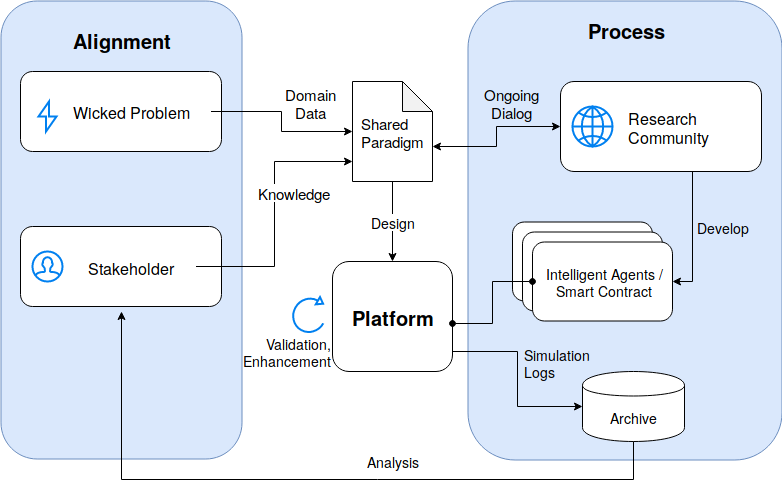
\includegraphics[width=1\linewidth]{./figures/competitive_benchmarking.png}
	\caption{Research Design following \protect\shortciteA{ketter2015competitive}}
	\label{figure:competitive_benchmarking}
\end{figure}

According to the IS Design Science principles introduced by Hevner, March, Park, and Ram \shortcite{hevner2008design}, 
the presented research design produce a viable artifact in the form of an open simulation platform, which depict a 
relevant real-world wicked problem. Due to the outcoming data produced by the simulation platform, 
it is possible to develop methods to evaluate the utility, quality and efficacy of the artifact. 
Moreover, the research provide a varifable contribution through the artifact, the open simulation platform, itself. 
The platform enables the investigation of possible solutions of unsolved problems and further, 
it removes the technical barriers for the use of the complex distributed ledger technology. 
Besides, the implementation of the platform is based on an appropriate selection of techniques. 
As stated in \ref{sec:Blockchain-based Energy Markets}, 
blockchains are a suitable technology to implement decentralized microgrid energy markets. 
In addition, the in \ref{sec:Distributed Resource Optimization} introduced distributed optimization 
algorithm achieve evidentially system optimality under a dynamic market-trading algorithm. 
Therefore, this research relies upon the application of rigorous methods and comply the requirement 
of the fifth guideline by \shortciteA{hevner2008design}. 
In addition, the platform enables the iterative search for an optimal design through the comparison 
of different produced solutions and is valuable to technology-oriented as well as management-oriented 
audiences. As a result, these research design also fulfil the seven research guidlines of 
the research framework introduced by \shortciteA{hevner2008design}. 


\section{Expected Contribution}
\label{sec:expected_contribution}

This research provides two different contributions. First, the fully decentralization of the introduced distributed optimization algorithm \shortcite{guo2007market}. 
The bundle-trading market grant access of any given trade to the market dealer. This, again, necessitates trust of the agents that it will use those resources according to the over-arching organizational goal. Due to the implementation of the market dealer by a smart contract, the technical implementation is public accesible. Moreover, all transactions of the market dealer to allocate the resources are transparent. Therefore, the behavior of the market dealer is comprehensible for every participant. Furthermore, it provides a high degree of security due to cryptographic encryption methods which are essential parts of the blockchain.
Second, the open simulation platform itself. From the scientific perspective, the platform is relevant due to the removal of existing technical barriers for practicioners in using complex distributed ledgers technologies. Therefore the platform facilitates researchers without a deep technically background to use those DLTs and incentivises to design and test their artifacts by using this platform. 
On the other hand, from a business perspective, this research is relevant to policy makers and energy suppliers. The platform allows stakeholders to get a better understanding of the dynamics of decentralized LEM and enables the testing and evaluating of policy options and implications. 

\clearpage

This chapter gives a short representation of the first platform design and the chosen technologies and frameworks. First, the Ethereum blockchain is implemented through Ganache. It is a personal local blockchain for the Ethereum development, which can be used to deploy smart contracts, develop decentralized applications, and run tests. Further, Ganache is available as a desktop application as well as a command-line tool. Next, the role of the market dealer is realized by a smart contract which is written in Solidity. This object-oriented programming language was especially designed for developing smart contracts that run on a Ethereum blockchain. The Solidity code is compiled to bytecode, which can be deployed into the blockchain. Moreover, the clients which constitute the different agents are implemented through the programming language Python. Python is a object oriented, high-level programming  language with a easy and simple to learn syntax. Therefore, the hurdles in modifying the client behavior are minimized. Finally, the clients using the Web3.py python library for the interaction with the Ethereum blockchain. 

\begin{figure}[htbp]
	\centering
	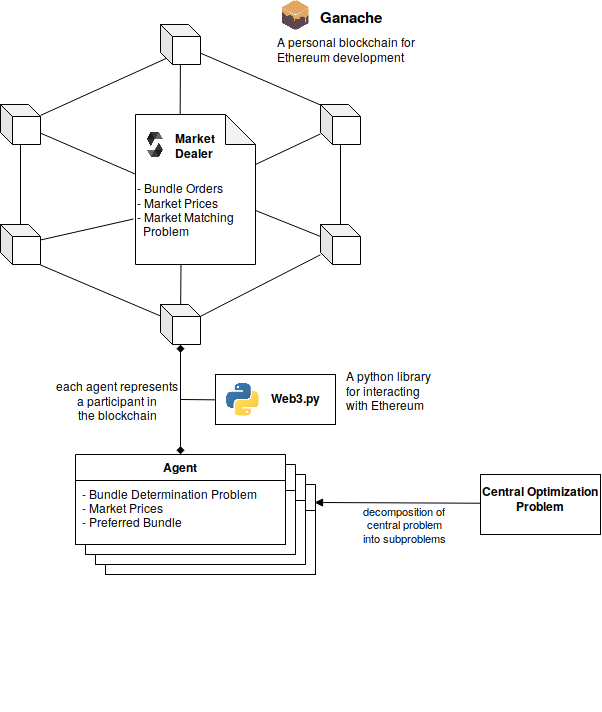
\includegraphics[width=.8\linewidth]{./figures/platform_architecture.png}
	\caption{Platform Design}
	\label{figure:paltform_architecture}
\end{figure}

\section{About Blockchain}

To begin with, this chapter will give an overview of the general purpose, the contained components and the fundamental functionality of a blockchain. 

\subsection{General Purpose}
In general, a blockchain can be described as a digital data structure that can be understand as a shared and distributed database, containing a continuous expanding and chronological log of transactions \shortcite{andoni2019blockchain}. Besides, various types like digital transactions, data records and executables can be stored in this digital data structure. The data transmission in a blockchain is comparable with copying data from one computer to another. However, the resulting challenge is that the system needs to ensure that the data is copied just once \shortcite{andoni2019blockchain}. For example, in the domain of cryptocurrencies, this is equal to sending a coin from one wallet to another. In this case, the system needs to validate that this coin is spended just once and there is no double-spending. A conventional solution for this problem is a third intermediary. To come back to the stated example, the third intermediary is represented by a traditional bank, which store, protect and continuously update the valid state of the ledger \shortcite{andoni2019blockchain}. But, in some cases central management is not practicable or reasonable. Reasons for this are possible intermediary costs or a high degree of trust of the users into the intermediary who operates the system. Further, central management has a significant disadvantage because of a single point of failure. Hence, the centralized system is fragile to technical problems as well to external malicious attacks \shortcite{andoni2019blockchain}.
Consequently, the main reason of bockchain technologies is the removal of such third trusted intermediaries through a distributed network of various users, who cooperating together to verify transactions and protect the validity of the ledger

\subsection{Architecture}
This subsection covers the architectural design of a blockchain and presents the contained components in detail. Due to the plurality of the blockchain technologies, each of the technology slightly differs in design and components. The following explanations are oriented torwards the Ethereum blockchain implementation, which is also used as the underlying ICT to implement the open simulation platform.

\subsubsection{World State}
\label{sec:world_state}
Referring to the \textit{Yellow Paper} by \shortciteA{wood2014ethereum}, Ethereum can be seen as a transaction-based state machine. What does that mean? At the beginning, Ethereums state machine starting with a so called \textit{"genesis state"}. This is analogous to a blank sheet. On this state, no transactions have happened on the network. Next, transactions are executed and the state of the Ethereum world changes into a new state. Further, transactions are executed incrementally and morph it into some final state. Consequently, the final state is accepted as the canonical version of the world of Ethereum and represents at any times the current state.

\begin{figure}[htbp]
	\centering
	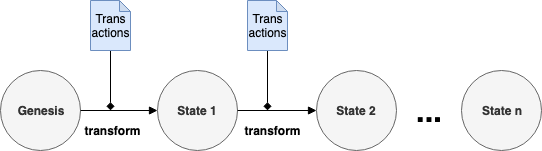
\includegraphics[width=.9\linewidth]{./figures/state_transition.png}
	\caption{World State: Transition of States}
	\label{figure:state_transition}
\end{figure}

In more detail, the world state arises out of a mapping of a key value pair for every account which exists on the Ethereum network \shortcite{wood2014ethereum}. The key constitutes the address of an Ethereum account and the value presents the account's state, which contains detailed information of this account. 
However, the world state is not stored on the blockchain itself. This mapping is stored and maintained in a modified data structure called a \textit{Merkle Patricia tree}. This tree is stored off-chain in a simple database backend (i.e. on a computer running an Ethereum client), also known as the \textit{state database} in the Ethereum world \shortcite{wood2014ethereum}. To get a better understanding of the operating principles of the blockchain, it is necessary to get an idea of how a \textit{Merkle Patricia tree} works. A \textit{Merkle Patricia tree} is a type of binary tree, which consists of a set of nodes. It has a large amount of 
\textit{leaf nodes}, containing the underlying data. Further, a set of intermediate nodes, where each node is the hash of its two children, and finally, one single root node, representing the top of the tree which is also build out of its two child nodes \shortcite{buterin2013next} \shortcite{wood2014ethereum}.
As mentioned before, the \textit{leaf nodes} contain the stored data by splitting these data into chunks. Afterwards, these chunks are splitted into buckets. Then, each bucket gets hashed and the same process repeats, traversing upwards the tree, until the total number of hashes remaining becomes only one and the root node is reached \shortcite{ethereum_blog}. 

\begin{figure}[htbp]
	\centering
	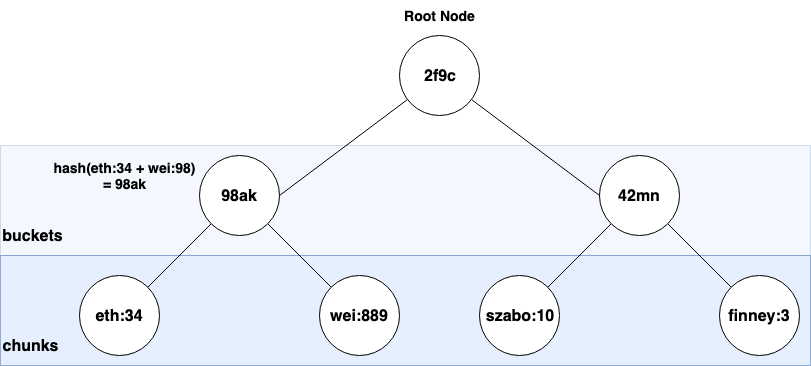
\includegraphics[width=.9\linewidth]{./figures/merkle_tree.png}
	\caption{Example of a Patricia Merkle tree}
	\label{figure:merkle_tree}
\end{figure}

Therefore, any change to the underlying data, stored in a \textit{leaf node}, causes a change of the hash of the node. Each parent's node hash depend on the data of its children. Due to this, any change to the data of a child node causes the parent hash to change. This procedure repeats traversing upwards until the root node. Hence, any change to the data at the leaf nodes effects the root hash \shortcite{ethereum_wiki}. 

\begin{figure}[htbp]
	\centering
	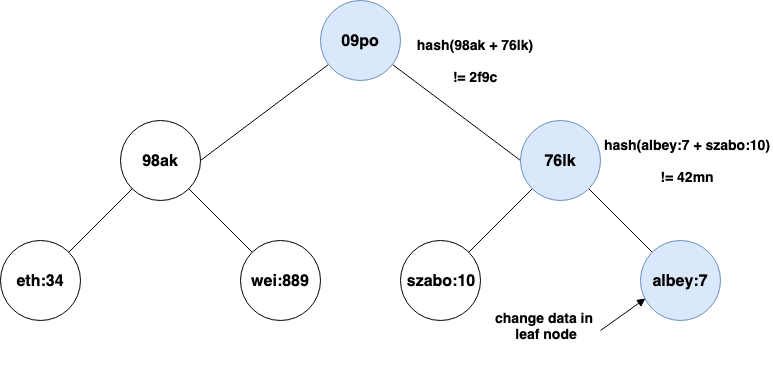
\includegraphics[width=.9\linewidth]{./figures/merkle_tree_change.png}
	\caption{Example of a data change in a leaf node}
	\label{figure:merkle_tree_change}
\end{figure}

Because of this characteristic, it is not necessary to compare the data of the entire tree. It is sufficient to compare the single root hash to ensure that all the data are the same. This property is very important, because it makes it possible to store only the hash of the root node to represent a state of the Ethereum world. 

\subsubsection{Block} 
\label{sec:block}
As described in section \ref{sec:world_state}, whenever transactions are executed, the state of the Ethereum world changes into a new state. Every state and the belonging transactions, which transform the prior state into the new state, is cumulated in a so called block. That means, states are represented by blocks. As you can see in figure \ref{figure:state_transition}, the history of the Ethereum world is a linkage of states, or in other words, blocks. That is where the name blockchain comes from. A blockchain is a sequence of blocks, which holds a complete list of transaction records \shortcite{zheng2017overview}. 
Moreover, a block is a collection of different relevant informations and consists of the \textit{block header} and the \textit{block body}, which contains the list of transactions. Following \textit{Ethereums Yellow Paper} by \shortciteA{wood2014ethereum}, the subsequent pieces of information are contained in the \textit{block header}:

\begin{description}
	\item[Parent Hash:] This is the hash of the parents block's header. Therefore, every block points to his ancestor. Due to this contained attribute, a chain arises out of the single blocks.
	\item[Beneficiary:] The miners address to which all block rewards from the successful mining of a block are transferred.
	\item[State Root:] This is the hash of the root node of the state tree, after a block and its transactions are finalized. As mentioned in section 
	\ref{sec:world_state}, the state tree is the one and only global state in the Ethereum world. It is used as a secure unqiue identifier for the state and the state root node is cryptographically dependent on all internal state tree data.
	\item[Transactions Root:] This is the hash of the root node of the transaction tree. This tree contains all transactions in the block body. In contrast to the state tree, there is a separate transactions tree for every block. 
	\item[Receipts Root:] Every time a transaction is executed, Ethereum generates a transaction receipt that contains information about the transaction execution. This field is the hash of the root node of the transactions receipt tree and like the transaction tree, there is a seperate receipt tree for every block.
	\item[Difficulty:] This is a measure of how hard it was to mine this block – a quantity calculated from the previous block’s difficulty and its timestamp
	\item[Number:] This is a quantity equal to the number of blocks that precede the current block in the blockchain.
	\item[Gas Limit:] This is a quantity equal to the current maximum gas expenditure per block. Each transaction consumes gas. The gas limit specifies the maximum gas that can be used by the transactions included in the block. It is a way to limit the number of transactions in a block.
	\item[Gas Used:] This is a quantity equal to the total gas used in transactions in this block.
	\item[Timestamp:] This is a record of Unix’s time at this block’s inception.
	\item[Nonce:] This is an 8-byte hash that verifies a sufficient amount of computation has been done on this block. Further, it is a number added to a hashed block that, when rehashed, meets the difficulty level restrictions. The nonce is the number that blockchain miners are solving for.
\end{description}

So far, we introduced Ethereum as a transaction-based state machine, transforming one state into another through the execution of transactions. Further, we explained how these individual states are stored and emphasises the meaning of these storage. Moreover, we pointed out that an Ethereum state is represented by blocks and described all relevant informations contained in it.
However, we didn't introduce how many transactions be part of a block and who build and validate a block? To answer this, we introduce the transaction object and his life cycle in depth.


\subsubsection{Transaction}
\label{sec:transaction}
To start with, a transaction is the basic method for Ethereum accounts to interact with each other. Further, in the Ethereum world exists two different types of transactions. Those, which result in a so called \textit{message call}, which can be seen as a traditional transaction, and those which result in a \textit{contract creation} \shortcite{wood2014ethereum}. 
Though, both different types of transaction share the following common attributes \shortcite{wood2014ethereum}:

\begin{description}
	\item[Nonce: ] This attribute is discontiguous of the block attribute. In contrast to the block attribute, the nonce of a transaction keep track of the total number of transactions that an account has executed. 
	\item[Gas Price: ] As mentioned in section \ref{sec:block}, each transaction consume gas. Gas can be seen as fees. This attribute presents the price per unit of gas for a transaction \footnote{A website to see current gas prices: https://ethgasstation.info/index.php}. 
	\item[Gas Limit: ] This attribute is similiar to the block attribute of the same name. In this case, it is a quantity equal to the current maximum gas expenditure per transaction.  
	\item[To: ] In case of a \textit{message call}, this attribute contains the address of the recipient. Otherwise, in case of a \textit{contract creation} this value remains empty. 
	\item[Value: ] In case of a \textit{message call}, this attribute contains the amount of Wei, which will be transferred to the recipient. In the case of a \textit{contract creation}, this value contains the amount of Wei as a intial endowment of the contract.
\end{description}

\subsubsection{Transaction Life Cycle}
\label{sec:transaction_lifecycle}
Next, the life cycle of a transaction will be outlined. We will take a simple \textit{message call} as an example and will pass through the entire flow of how this transaction gets executed and permanently stored on the blockchain. During this process, many basic concepts of a blockchain will be introduced. 

To begin with, someone want to send an abitrary amount of ether to someone else. 
Consequently, a transaction with the respective attributes, which are stated 
in section \ref{sec:transaction}, will be created. As a first step, this transaction 
will be signed. That means, the one who wants to execute the transaction needs to proof the 
ownership of the account. Otherwise, someone else could execute a transaction on your behalf. 
The way to proof this is by signing the transaction with the corresponding private
key of this account \shortcite{transaction_life_cycle}. 
Next, the signed transaction is submitted to the related Ethereum node. 
Then, the node will validate the signed transaction. 
After a successful validation, the node will send the transaction to 
it's peer nodes, who again send it to their 
peer nodes and so on \shortcite{transaction_life_cycle}. 
As soon as the transaction is broadcast to the network, 
the related node will declare a transaction id, which is the hash 
of the signed transaction and can be used to track the 
status of the transaction \footnote{A Website to track transactions: https://etherscan.io/}. 

\begin{figure}[htbp]
	\centering
	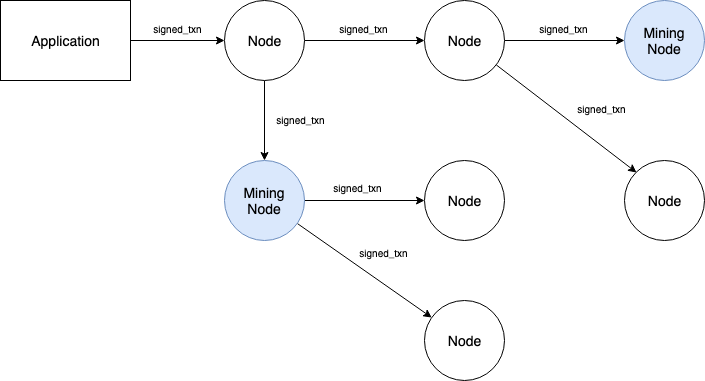
\includegraphics[width=.9\linewidth]{./figures/node_network.png}
	\caption{Node network demonstrating a transaction broadcast}
	\label{figure:node_network}
\end{figure}

\clearpage

Further, figure \ref{figure:node_network} describes a Ethereum network. 
As you can see, it contains a mix of miner nodes and non miner nodes. 
The non miner nodes can be distinguished into different types of nodes with different 
behavior, which are explained in detail in section \ref{sec:nodes}. 
The miner nodes are the ones who processing transactions into blocks \shortcite{transaction_life_cycle}. 

Mining nodes contain and maintain a pool of transactions where they collect incoming transactions. 
They sort the transactions by gas price. 
However, there are no specific rules how the nodes sort the transactions. 
A common configuration is to sort the transaction by gas price in a descending order to 
optimize for a higher pay \shortcite{transaction_life_cycle}.

\begin{longtable}{c|c}
	\hline
	Signed Transaction & Gas Price \\
	\hline
	hashOfTransaction1 & 15 Gwei \\
	hashOfTransaction2 & 13 Gwei \\
	hashOfTransaction3 & 11 Gwei \\
	hashOfTransaction4 & 10 Gwei \\
	hashOfTransaction5 & 7 Gwei \\
	\hline
	\caption{Transaction Pool of Mining Node}
	\label{table:sorted_gas_prices}
\end{longtable} 

Further, the mining node takes transactions from the pool and processes them into a pending block. 
Moreover, a block can only contain a certain number of transactions due to the block 
attribute \textit{gas limit}, mentioned in section \ref{sec:block}. 
That means, the mining node can only process so many transactions into one 
block until the gas limit is reached \footnote{A website to see 
current attributes: https://ethstats.net/}. For example, 
imagine that the current \textit{gas limit} of a block is 28 Gwei. 
Next, we look at the transaction pool of a mining node in 
table \ref{table:sorted_gas_prices}. As you can see, two blocks are 
required to process all transactions from the pool. The first two transactions 
are contained in the first block. Furhtermore, the second block contains the remaining 
three transactions. 
So far, it is described how a pending block will be created and the transaction 
limit of a block is explained. In the next section \ref{sec:mining}, 
the process of a pending block to a valid block is outlined in depth. 
Finally, after the validation process of a block is finished successfully, 
the life cycle of a transaction is terminated. In other words, the transaction is anchored 
in the blockchain and modified the world state as mentioned in section \ref{sec:world_state}.

\subsubsection{Mining}
\label{sec:mining}
In this section, the stteps of the validation process of a pending block will be described. 
In general, each mining node in the network can generate or propose a block. 
The emerging question is, which node build the new block and how will the newly 
generated block accepted by the remaining network members? 
This process is called \textit{consensus mechanism}.
It exists a lot of various consensus algorithms, each of them provides different features,
advantages and disadvantages. 

To a large extent, the key perfomance drivers of a blockchain
like transaction speed, scalability and security depending on the embedded consensus algorithm \shortcite{andoni2019blockchain}. 
In this section, we will expound the \textit{Proof of Work (PoW)} mechanism, 
which is at the time of this writing the current strategy in the Ethereum blockchain 
implementation for reaching consensus. 
\textit{Proof of Work} enables a high scalability in terms of the number 
of nodes and clients \shortcite{vukolic2015quest}, whereas it provides a poor transaction speed and a high 
power consumption due to the solving of a cryptographical puzzle, which requires 
significant computational effort \shortcite{andoni2019blockchain}. 

% erklärung crypthograpgical puzzle
The \textit{PoW} is a random process which is not predictable and therefore only solvable through a 
trial and error approach \shortcite{bitcoin_wiki_pow}. 
All mining nodes compete with each other and the goal is to achieve a hash output that 
is lower than a given specified target \shortcite{andoni2019blockchain}.
The hash output includes and comprises out of the \textit{Parent Hash}, \textit{Transaction Root} and
\textit{Nonce}, which are all part of the block headers data, mentioned in \ref{sec:block}.
However, the \textit{Parent Hash} and \textit{Transaction Root} are given and immutable, thus the \textit{Nonce}
is the value that all the mining nodes are solving for \footnote{A interactive blockchain demo: https://anders.com/blockchain/}.
Consequently, the mining nodes modify the \textit{Nonce} until the hash output is lower than the required target \shortcite{andoni2019blockchain}.
The following pseudocode in listing \ref{lst:pow_mechanism} will illustrate the \textit{PoW} procedure:

\vspace{7mm}
\begin{lstlisting}[label={lst:pow_mechanism}, caption={Pseudocode for PoW mechanism}]
	targetValue = 00005cdf6d384113165841052dfd4638eaf756ac
	parentHash = abbecf2d59eacbde676c3f1f0bfcf124f8c68209
	transactionRoot = 917c631e5ee59596859910759c8ed76a21252010
	nonce = 1
	valid = False

	while(not valid):
			hashOutput = sha256(parentHash+transactionRoot+nonce)
		
			if(hashOutput <= targetValue):
					valid = True
			else:
					nonce += 1

\end{lstlisting}
\clearpage

Finally, when one mining node successfully calculated the \textit{Nonce} and therefore reaches the target value, 
it broadcasts the block to all other mining nodes in the network. Now, all other nodes mutually validate the correctness of the hash value
by recalculating the hash output and verifying if it is lower then the target value. 
If the block is validated through all other mining nodes, all nodes will append this new block to their own blockchains \shortcite{zheng2017overview}.  

% erklärung multiple chains
Considering, the network is decentralised and the simultaneous generation of valid blocks is possible when multiple nodes find 
the suitable \textit{Nonce} at a nearly same time \shortcite{zheng2016blockchain}. In this case, branches will be generated as shown in figure \ref{figure:blockchain_branches}

\begin{figure}[htbp]
	\centering
	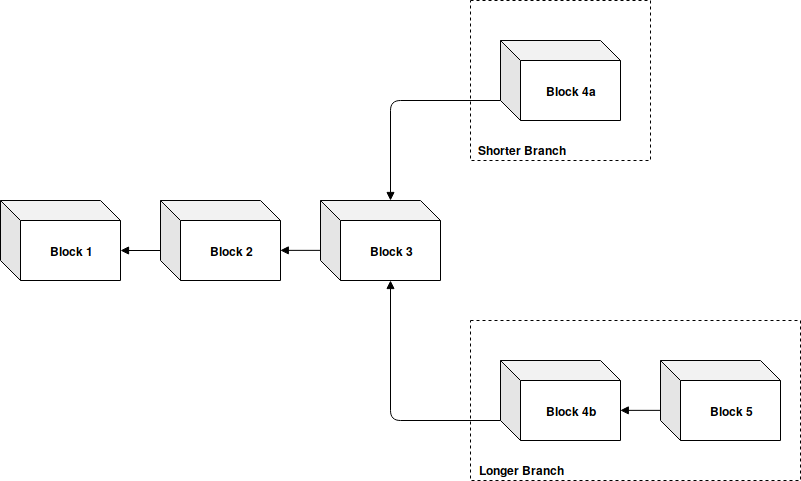
\includegraphics[width=.9\linewidth]{./figures/blockchain_branches.png}
	\caption{Scenario of Blockchain Branches}
	\label{figure:blockchain_branches}
\end{figure}

Nevertheless, it is unlikely that two competing branches will generate the next block simultaneously again. 
In the \textit{PoW} protocol, the longer branch is judged as the authentic one. 
In figure \ref{figure:blockchain_branches}, two branches arised out of 
two simultaneous valided blocks \textit{Block 4a} and \textit{Block 4b}. 
After that, all mining nodes accept both branches and start working on 
the next consecutive block until a longer branch is found \shortcite{andoni2019blockchain}. 
As you can see in figure \ref{figure:blockchain_branches}, \textit{Block 4b} and \textit{Block 5} forms the longer 
chain, therefore all miners on the branch with \textit{Block 4a} will switch to 
the longer branch \shortcite{zheng2017overview}. 

To sum up, this section joins and completes the previous section \ref{sec:transaction_lifecycle}.
The consensus mechanism \textit{PoW} is described and outlined in pseudocode, whereby
the validation process of new generated blocks is explained and illustrated.
\clearpage

\subsubsection{Ethereum Clients}
\label{sec:nodes}

First of all, the expressions Ethereum client and Ethereum node can be used interchangeable. 
As mentioned earlier in the previous section \ref{sec:transaction_lifecycle} 
and illustrated in the figure \ref{figure:node_network}, clients can be distinguished into different types. 
This section will describe the concept of an Ethereum client in general and will give a brief overview of the different
types.

In general, an Ethereum client is a software application 
that implements the Ethereum specification, which is specified in the Ethereum yellow paper \shortcite{wood2014ethereum}.
A client communicates over the peer-to-peer network with other Ethereum clients.
Although these clients can be implemented in different programming languages, they all communicate through
the standardized Ethereum protocol, wherefore they are able 
to operate and interact with the same Ethereum network. \shortcite{antonopoulos2018mastering}. 

Since the Ethereum blockchain is not officially implemented in a particular programming language, 
following a list of the current main implementations of the Ethereum protocol:

\begin{itemize}
	\item \texttt{Parity}, written in Rust
	\item \texttt{Geth}, written in Go
	\item \texttt{cpp-Ethereum}, written in C++
	\item \texttt{pyethereum}, written in Python
	\item \texttt{Harmony}, written in Java 
\end{itemize}

However, while all clients differ from each other, they share some fundamental features \shortcite{ethereum_clients}.

First, each is able to join the peer-to-peer Ethereum network. 
Next, they all synchronizing a local copy of the blockchain.
There are a few modes of synchronizing, which comes with miscellaneous advantages and disadvantages, 
which will be outlined later on. Moreover, it makes a significant difference 
for the health and resilience of the decentralised network. 
Lastly, each client is also capable of broadcasting new transactions to the network and creating and 
managing accounts \shortcite{ethereum_clients}.

As mentioned above, there are differences in client behavior regarding to the synchronizing modes. 
In general, the clients can be distinguished into two different types, the so called \textit{full node} and 
\textit{light node}. 

\paragraph{Full Node:} A full node will download all history data peer-to-peer from
another full node. This requires a significant amount of hardware and bandwith resources \shortcite{antonopoulos2018mastering}.
Afterwards, it will simulate every transaction in the ledger
and execute the whole deployed source code to recalculate the state of each existing block \shortcite{ethereum_clients}.
Therefore, the amount of independently operating and geographically dispersed full nodes 
is a crucial and very important indicator for the health, resilience and 
censorship resistance of a blockchain \shortcite{antonopoulos2018mastering}. 
However, a full node is not necessarily a mining node. It authoritatively validates all transactions, but 
to participate in the mining competition, an additional software called \textit{ethminer}
 is needed \footnote{GPU Mining Worker: https://github.com/ethereum-mining/ethminer}

\paragraph{Light Node:} To begin with, a light node is not a separate piece of software from the clients that 
run a full node. The difference lies in the \textit{light} mode for synchronization. 
In contrast to a full node, a light node only synchronize the block headers and the 
current state of the chain \shortcite{ethereum_light_node}.
Anyway, a light node lacks the ability to run transactions throughout the history of the 
whole blockchain. For this reason, it does not contribute to the health and resilience of 
the network like a full node and traditionally cannot act as a mining node \shortcite{ethereum_clients}. 
In addition, a light node has some further limitations. For instance, they are not 
capable to monitor pending transactions from the network and the hash of a transaction
is not sufficient to locate the transaction. Moreover, to perform certrain types of operations,
a light node relies on requests to full nodes, whereby they can be far slower to query the chain \shortcite{ethereum_light_node}.


\subsubsection{Smart Contract}

This section deals with smart contracts in the Ethereum world and based 
entirely on the book \textit{Mastering Ethereum} by \shortciteA{antonopoulos2018mastering}.
First of all, the term smart contract is a bit misleading, since Ethereum smarts contract 
are neither smart nor legal contracts. However, how can a Ethereum smart contract be defined?
A Ethereum smart contract is an immutable comuputer program that runs deterministically in the context of an
Ethereum Virtual Machine (EVM) as part of the networkprotocol. To go into the definition in more detail, 
immutable means, that once the contract is deployed into the blockchain, it is not possible to make any
changes in the source code. The only way to modify the contract is to deploy a whole new instance. 
Further, deterministic means that the result of the execution is the same for all who run it, 
depending on the context of the transaction that initiated its execution and the state of the blockchain
at the moment of execution.
As already mentioned in section \ref{sec:transaction}, in the Ethereum world exists two different types of transactions.
Those which result in a message call, and those which result in a contract creation. 
That means, smart contracts are deployed through special contract creation transactions into the blockchain. 
The special thing about these transactions is that the recipient of the transaction remains empty, whereby the transaction
will be send to a special destination address called \textit{zero address (0x0)}. Each contract is identified and reachable via
a common Ethereum address, which can be used in a transaction as the recipient to send funds to the contract or to call 
one of the contract functions. Anyway, in contrast to an externally owned account, there are no keys associated with 
an account of a smart contract. For this reason, the creator of a smart contract does not have any special rights at the 
protocol level. Although, it is possible to get those special rights if you explicitly 
specified them in the source code of the contract.
Furhtermore, contracts are only active and run if they called by a transaction. 
A contract is able to call another contract and so on, but nevertheless, 
the first call have always come from an externally owned account. 
A contract will never run on his own or in the background. Additionally, contracts are not executed in parallel.
They will always executed consecutively, hence the Ethereum blockchain can be considered as a single-threaded machine. 
Finally, it should be noted that transactions are atomic regardless of how many contracts they call. Transactions execute in
their entirety and any changes in the global state are only recorded if all executions terminates successfully. 
If the executions fails, all the changes in state are reverted as if the transaction never ran. Anyhow, a failed
execution of a transaction is recorded as having been attempted. Moreover, the gas fees spent for the execution is withdrawn
from the originating account.

\clearpage

\section{Linear Programming}
\label{sec:linear_progamming}
This section will give an introduction into the basics of mathematical linear programming
and linear programming duality.
It will present the purpose and necessity of optimization models and will give
an example of how an optimization model is constructed. 

To begin with, optimization models try to define in mathematical terms, the goal
of solving a problem in the best or optimal way. 
This can be applied in many different areas, for example, it might mean running a business to 
maximize profit, designing a bridge to minimize weight or selecting a flight plan for an aircraft
to minimize time or fuel use \shortcite{griva2009linear}. 
The use case of solving an optimization problem optimally is so ubiquitous, 
that optimization models are used in almost every area of application \shortcite{griva2009linear}.
Often it is not possible or economically feasible to make decisions without the help
of such a model. Due to the excellent improvements in computer hardware and software
in the last decades, optimization models became a practical tool 
in business, science and engineering \shortcite{griva2009linear}. 
Finally, it is possible to solve optimization problems with a huge set of variables. 

Further, linear optimization, also known as a \textit{linear program (LP)}, refers to the optimization
of a linear function with the decision variables, $x_{1}, ..., x_{n}$ subject to 
linear equality or inequality constraints. 
As presented by \shortciteA{bichler2017market}, in canonical form 
a linear optimization model is given as:

\begin{equation*}
    \begin{array}{ll@{}ll}
        \text{max}  & \displaystyle\sum\limits_{j=1}^{n} c_{j}x_{j} &\\
        \text{s.t.}& \displaystyle\sum\limits_{j=1}^{n} a_{ij}x_{j} \leq b_{i},  &&i=1 ,..., m\\
                    &                        x_{j} \geq 0, &&j=1 ,..., n
    \end{array}
\end{equation*}

However, a LP can be modeled in different forms. It is also possible 
to write a model in the matrix-vector notation. To represent the above model in this form, letting
$x=(x_{1}, ..., x_{n})^{T}$, $c=(c_{1}, ..., c_{n})^{T}$, $b=(b_{1}, ..., b_{m})^{T}$
and name the matrix of the coefficients $a_{ij}$ by $A$. As introduced by \shortciteA{griva2009linear},
the model becomes:

\begin{equation*}
    \begin{array}{ll@{}ll}
        \text{max}  & \displaystyle c^{T}x &\\
        \text{s.t.}& \displaystyle Ax \leq b&\\
                    &                        x \geq 0
    \end{array}
\end{equation*}

\clearpage
In general, the objective function of a linear model is either minimized or maximized.
Additionally, the constraints may include a combination of inequalities and equalities
and the variables are unrestricted or restricted in sign \shortcite{bichler2017market}.

\subsection{Duality Theory}
\label{sec:duality_theory}
In addition, for every LP exists another problem, which
is called the \textit{dual} of the original linear problem, also known as the 
\textit{primal} \shortcite{bichler2017market}.
In the dual, the roles of variables and constraints are reversed. 
That means, every variable of the primal becomes a constraint in the dual,
and every constraint in the primal becomes a variable in 
the dual \shortcite{griva2009linear}.
For instance, if the primal has $n$ variables and $m$ constraints, the dual
will have $m$ variables and $n$ constraints. Further, the primal objective coefficients 
are the coefficients on the right-hand side of 
the dual, and vice versa.
Finally, the transposed coefficient matrix of the primal constitutes the matrix in the 
dual \shortcite{griva2009linear}.
To give an example of a primal and the corresponding dual LP,
the representation by \shortciteA{bichler2017market} is considered:

\begin{equation}
    \tag{primal}
    \begin{array}{ll@{}ll}
        \text{min}  & \displaystyle c^{T}x &\\
        \text{s.t.}& \displaystyle Ax \geq b  &\\
                    &                        x \geq 0
    \end{array}
\end{equation}

\begin{equation}
    \tag{dual}
    \begin{array}{ll@{}ll}
        \text{max}  & \displaystyle b^{T}y &\\
        \text{s.t.}& \displaystyle A^{T}y \leq c &\\
                    &                        y \geq 0
    \end{array}
\end{equation}


Next, the motivation of the duality theory can be explained by the issue of trying to find 
bounds on the value of the optimal solution to a LP. 
If the primal is a minimization problem, the dual represents a lower bound
on the value of the optimal solution, otherwise, if the primal is a maximization problem,
the dual represents an upper bound \shortcite{bichler2017market}.
To illustrate the concept and motivation of duality theory more tangibly, an example stated by 
\shortciteA{bichler2017market} is given. 
In an application, the variables in the primal linear problem stand for consumer products and
the objective coefficients represent the profits linked to the production of those consumer products. 
In this case, the objective in the primal describes directly the relation between a change
in the production of the products and profit. Whereas, the constraints in the primal 
describe the availability of raw materials. Consequently, an increase in the availability of 
raw materials needed for the production of the consumer products enables an increase in production,
and finally an increase in the overall profit. 
However, the primal problem does not outline this relationship reasonable. Hence, one of 
the benefits of the dual is to properly show the effect of changes in the constraints on the
value of the objective. Due to this, the variables in a dual LP often called 
\textit{shadow prices}, since they describe the hidden costs associated with the constraints. 

\subsubsection{Weak Duality Theorem}
As stated in the section before (\ref{sec:duality_theory}), the \textit{dual} problem 
provides, depending on maximization or minimization problem, lower and upper bounds for 
the \textit{primal} objective function. Referring to \shortciteA{vanderbei2015linear},
this result is true in general and is described as the \textit{Weak Duality Theorem}:

\begin{theorem}
    If $x$ is feasible for the primal and 
    $y$ is feasible for the dual, then:

    \begin{equation*}
        \begin{array}{ll@{}ll}
            \displaystyle c^{T}x \leq b^{T}y&\\
        \end{array}
    \end{equation*}    

\end{theorem}

Regarding to \shortciteA{griva2009linear}, there are some logical corollaries 
of the Weak Duality Theorem:

\begin{corollary}
    If the primal is unbounded, then the dual is infeasible. 
    If the dual is unbounded, then the primal is infeasible.
\end{corollary}

\begin{corollary}
\label{strong_duality_corollary}
    If $x$ is a feasible solution to the primal, 
    $y$ is a feasible solution to the dual,
    and $c^{T}x = b^{T}y$, then x and y are optimal for their respective problems.
\end{corollary}

\subsubsection{Strong Duality Theorem}
\label{sec:strong_duality_theorem}
Concerning corollary \ref{strong_duality_corollary}, it is possible to verify if 
the points x and y are optimal solutions, without solving the corresponding LPs. 
Furthermore, this corollary is also used in the proof of strong duality \shortcite{griva2009linear}. 
The \textit{Strong Duality Theorem} describes, that for linear programming there 
is never a gap between the primal and the dual 
optimal objective values \shortcite{vanderbei2015linear}.

\begin{theorem}
    If  the primal problem has an optimal solution $x^{*}$,
    then the dual also has an optimal solution $y^{*}$,
    such that:

    \begin{equation*}
        \begin{array}{ll@{}ll}
            \displaystyle c^{T}x^{*} = b^{T}y^{*}&\\
        \end{array}
    \end{equation*}    

\end{theorem}

\subsubsection{Simplex-Method}
This subsection will give a brief introduction to the \textit{simplex-method}. 
To start with, in the field of linear programming, the simplex-method 
is the most widely used algorithm. 
This method was developed around 1940 and had several competitors at that time.
However, the algorithm was able to assert itself due to its efficiency. \shortcite{griva2009linear}
In general, the simplex-method is an iterative algorithm, used to solve 
a LP \shortcite{griva2009linear}. To apply the algorithm to a LP, 
it must be in standard form \shortcite{Luenberger2008}. According to \shortciteA{griva2009linear}, 
we consider the following LP:

\begin{equation*}
    \begin{array}{ll@{}ll}
        \text{min}  & \displaystyle z = -x_{1} - 2x_{2} &\\
        \text{s.t.}& \displaystyle - 2x_{1} + x_{2} \leq 2 &\\
                    & \displaystyle - x_{1} + 2x_{2} \leq 7 &\\
                    & \displaystyle  x_{1} \leq 3 &\\
                    &                        x_{1}, x_{2} \geq 0
    \end{array}
\end{equation*}

Next, we give an example to illustrate how to convert a LP into standard form.
To achieve that, the so-called \textit{slack variables} will be added, which represents the 
difference between the right-hand side and the left-hand side. 

\begin{equation*}
    \begin{array}{ll@{}ll}
        \text{min}  & \displaystyle z = -x_{1} - 2x_{2} &\\
        \text{s.t.}& \displaystyle - 2x_{1} + x_{2} + x_{3} = 2 &\\
                    & \displaystyle - x_{1} + 2x_{2} + x_{4} = 7 &\\
                    & \displaystyle  x_{1} + x_{5} = 3 &\\
                    &                        x_{1}, x_{2}, + x_{3}, + x_{4}, + x_{5} \geq 0
    \end{array}
\end{equation*}


Finally, with the LP in standard form, the idea of the simplex-method
is to iteratively proceed from one basic feasible solution to another \shortcite{Luenberger2008}.
Thereby, it always looks for a feasible solution which is better than the one before. 
The definition of better, in this case, depends on the nature of the linear problem. 
The process is performed until a solution is reached, which cannot 
be improved anymore. In the end, this final solution is then an optimal solution \shortcite{vanderbei2015linear}. 


\clearpage







%%%%%%%%%%%%%%%%%%%%%%%%%%%%%%%%%%%%%%%%%%%%%%%%%%%%%%%%%%%%%
%APPENDICES
%%%%%%%%%%%%%%%%%%%%%%%%%%%%%%%%%%%%%%%%%%%%%%%%%%%%%%%%%%%%%

\clearpage
\appendix
\renewcommand*{\thesection}{\Alph{section}}\textbf{}

% APPENDIX A
\section{Appendix}

\subsection{Additional Off-chain Dealer Description}
\label{appendix:additional_offchain}

\begin{lstlisting}[float=htbp, label=lst:creation_mmp, caption=Creation of MMP, language=Python]
    def create_mmp(self):
        bundles = [order.get_concatenated_bundles() for order in self._order_handler.get_all_orders()]
        bids = [order.get_concatenated_bids() for order in self._order_handler.get_all_orders()]

        try:
            TARGET_COEFS = np.hstack(bids) * (-1)  # create target coef vector

            self._mmp_amount_variables = np.size(TARGET_COEFS)  # set amount of variables
            mmp_coefs = np.hstack(bundles)
            var_leq_one_coefs = np.identity(self._mmp_amount_variables, dtype=float)  # create constraint matrix for y<=1
            var_geq_zero_coefs = np.identity(self._mmp_amount_variables, dtype=float) * (-1)  # create constraint matrix for y>=0
            mmp_bounds = self._resource_inventory
            var_leq_one_bounds = np.ones(self._mmp_amount_variables, dtype=float)
            var_geq_zero_bounds = np.zeros(self._mmp_amount_variables, dtype=float)

            CONSTRAINT_COEFS = np.concatenate((mmp_coefs, var_leq_one_coefs, var_geq_zero_coefs), axis=0)  # create final constraint matrix
            CONSTRAINT_BOUNDS = np.concatenate((mmp_bounds, var_leq_one_bounds, var_geq_zero_bounds))  # create final bounds matrix

            self._mmp_constraint_coefs = CONSTRAINT_COEFS
            self._mmp_constraint_bounds = CONSTRAINT_BOUNDS
            self._mmp_target_coefs = TARGET_COEFS

        except ValueError as error:
            print('Creation of MMP failed!')
            print(error)
\end{lstlisting}

\begin{lstlisting}[float=htbp, label=lst:solving_mmp, caption=Solving of MMP, language=Python]
    def solve_mmp(self):
        solvers.options['show_progress'] = False
        sol = solvers.lp(matrix(self._mmp_target_coefs), matrix(self._mmp_constraint_coefs), matrix(self._mmp_constraint_bounds))
        self._mmp_values = np.array([float('%.2f' % (sol['x'][i])) for i in range(self._mmp_amount_variables)])
        self._mmp_duals = np.array([float('%.2f' % entry) for entry in sol['z']])
        self._mkt_prices = np.array([float('%.2f' % (sol['z'][i])) for i in range(self._shared_resource_size)])
\end{lstlisting}





%%%%%%%%%%%%%%%%%%%%%%%%%%%%%%%%%%%%%%%%%%%%%%%%%%%%%%%%%%%%%
%BIBLIOGRAPHY
%%%%%%%%%%%%%%%%%%%%%%%%%%%%%%%%%%%%%%%%%%%%%%%%%%%%%%%%%%%%%

\clearpage
\renewcommand*{\thesection}{}\textbf{}

\bibliographystyle{apacite}
\bibliography{references.bib}


\end{document}